\section{Arquitetura}

Com base na análise do projeto, e nos requisitos que foram levantados
como necessários, a arquitetura cliente-servidor é plausível como
modelo para o produto que pretendemos entregar.
Esta arquitetura é composta por duas aplicações distintas:
\begin{itemize}
\item Uma aplicação \gls{frontend}, focada na interação com o usúario
  e apresentação de dados de uma forma agradável e intuitiva. Esta
  aplicação será implementada em JavaScript, com o \gls{framework} React
  Native, e disponibilizada para as plataformas iOS e Android.
\item Uma aplicação \gls{backend}, que será responsável por tratar os
  dados coletados no \gls{frontend} e disponibilizar as informações
  que serão mostradas aos usuários. Como esta aplicação requer uma
  lógica de servidor, estabilidade e ampla disponiblidade, esta
  aplicação será implementada em Java, com uso do \gls{framework} Spring
  Boot, que abstrai a criação de um servidor.
\end{itemize}
Podemos ver na \autoref{fig:cli-srv} uma respresentação desta
arquitetura.

\begin{figure}[h]
  \centering
  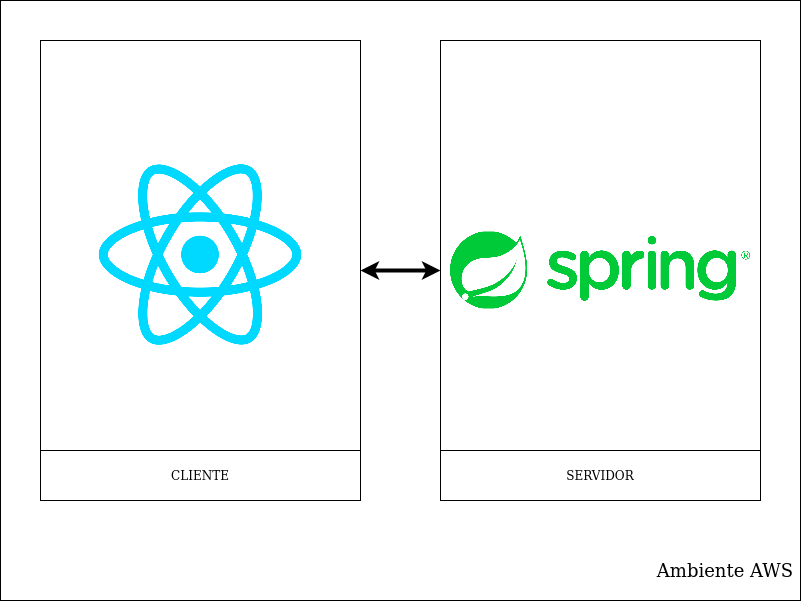
\includegraphics[scale=0.4]{lixt}
  \caption{Arquitetura Lixt}
  \label{fig:cli-srv}
\end{figure}

A comunicação entre estes serviços será feita com o uso do protocolo
\label{sig:https}\hyperlink{s:http}{HTTPS}, que permite a aplicação
cliente realizar chamadas ao servidor através de urls, seja para
buscar informações para apresentar ao usuário ou postar informações
coletadas dele. O \gls{\gls{framework}} Spring, além de abstrair a implementação
da lógica de um servidor, implementa \emph{listeners} para estas urls,
auxiliando a criação de pontos na aplicação do servidor focados na
comunicação com a aplicação cliente.

O uso do protocolo HTTPS oferece alguamas vantagens a aplicação
\gls{frontend}, que não precisa esperar uma solicitação ao
\gls{backend} ser finalizada antes de realizar outras solicitações,
aumentando a repsonsividade da aplicação cliente. Para além disso,
quando combinada ao modelo \label{sig:rest}\gls{REST} na
construção da \label{sig:API}\gls{API}, o protocolo HTTP
oferece meios eficientes para que as aplicações se comuniquem.

Como plataforma de servidor, o serviço AWS será utilizado, uma vez que
é oferecida de maneira gratuita para a realização deste projeto, e nele
serão armazenadas algumas instâncias da aplicação \gls{backend}.
Esta redundância é necessária como forma de garantir a estabilidade do
sistema, de forma que sempre haja alguma disponível para o
processamento de novas requisições, e, em caso de falha numa delas, o
serviço não seja interrompido aos usuários.

%%% Local Variables:
%%% mode: latex
%%% TeX-master: "../../desenho"
%%% End:
